\chapter{Background}
In this chapter, we review and introduce some essential concepts used in this work. First, we give a short introduction to the Haskell Programming Language in Section~\ref{sec:haskell}. Later, we briefly describe the fundamentals of concurrency in Section~\ref{sec:conc}. Finally, we present the primitives and constructors for concurrent programming in Haskell in Section~\ref{sec:haskell-conc}.

\section{Haskell}\label{sec:haskell}
Haskell is a \emph{purely functional} programming language. Being functional means that functions are the building blocks of programs written in this language. Being pure means that no side-effect happens when evaluating a function. These two characteristics together make Haskell fundamentally different from imperative programming languages. In imperative programming languages, a program is expressed as a sequence of instructions that mutate data. In Haskell, a program is expressed as a composition of expressions where all state is controlled by passing arguments to function calls and returning values from them. Also, having no side-effect guarantees that, in a given execution context, a function executed with a given argument will always produce the same result. This property is known as \emph{referential transparency}. It enforces that a program's behavior cannot depend on history, which improves reasonability.

Haskell is also a \emph{lazy} programming language. Lazy refers to a non-strict evaluation strategy also known as \emph{call-by-need}. This strategy delays the evaluation of an expression until its value is needed. It avoids repeated evaluations, which can lead to performance improvements. This strategy also makes it possible to construct potentially infinite data structures.

Regarding programming style, \emph{recursion} is the norm in Haskell since regular iterative loops require state mutation. To make it easier to express recursive functions, Haskell also has \emph{pattern matching}. In \autoref{code:fact}, we can see an example of a recursive function using pattern matching. Line 1 is the base case, when the \texttt{factorial} receives zero as an argument, and Line 2 is the general case.

\begin{listing}
  \caption{A recursive factorial function}
  \begin{minted}{haskell}
factorial :: Int -> Int
factorial 0 = 1
factorial x = x * factorial (x - 1)
  \end{minted}
  \label{code:fact}
\end{listing}

Functions in Haskell can be \emph{polymorphic}, which means that a function can be generalized to work with multiple types instead of a single one. Other programming languages have similar features such as \emph{generics} in Java and \emph{templates} in C++. \autoref{code:poly} shows an example of a polymorphic function that can reverse a list of any type. In this example, \texttt{t} is a \emph{parametric type} used to bind the input type to the output type of \texttt{reverse}. It reads: \texttt{reverse} receives a list of any type and returns a list of the same type as the input. This kind of polymorphism is known as \emph{parametric polymorphism}~\cite{cardelli:1985}.

\begin{listing}
  \caption{A polymorphic function to reverse a list}
  \begin{minted}{haskell}
reverse :: [t] -> [t]
reverse l = rev l []
  where
    rev []     a = a
    rev (x:xs) a = rev xs (x:a)
  \end{minted}
  \label{code:poly}
\end{listing}

Another characteristic of Haskell is that functions are values. This means that a function can receive other functions as arguments, and can also be the result of a function evaluation. This feature is known as \emph{high-order functions}. It enables very popular functional patterns such as \texttt{map}, \texttt{filter}, and \texttt{reduce}. In \autoref{code:map}, we can see \texttt{map} implemented in Haskell. It returns the list obtained by applying the provided function to each element of the input list.

\begin{listing}
  \caption{The \texttt{map} function}
  \begin{minted}{haskell}
map :: (a -> b) -> [a] -> [b]
map _ []     = []
map f (x:xs) = f x : map f xs
  \end{minted}
  \label{code:map}
\end{listing}

In Haskell, a developer can also extend the built-in primitive types by defining new \emph{abstract data types}. \autoref{code:tree} shows an example defining the \Tree data type and the function \texttt{depth} to calculate the depth of the tree. As this example shows, the parametric polymorphism also works for abstract data types. Here, \Tree has two constructors \texttt{Node} and \texttt{Empty}, where the first one holds three elements: the value of the node, the, left and right sub-trees. Pattern matching can be used to walk through a \Tree as shown in Lines 5 and 6.

\begin{listing}
  \caption{A data type for binary tree and a function to calculate its depth}
  \begin{minted}{haskell}
data Tree t = Node t (Tree t) (Tree t)
            | Empty

depth :: Tree t -> Int
depth Empty        = 0
depth (Node _ l r) = 1 + max (depth l) (depth r)
  \end{minted}
  \label{code:tree}
\end{listing}

There is also a concept called \emph{type classes} that enhances the definition of new types in Haskell. A type class is similar to an interface in Java. It defines a set of functions that can be applied to a particular type. This set of functions can be seen as a protocol to which a type must comply. So to instantiate a type class, a type must have its own implementation of each function defined by the protocol. As interfaces in Java, type classes were designed as a way for implementing ad hoc polymorphism in Haskell. The main difference between the two concepts is that type class instances are declared separately from the declaration of the corresponding types; while in Java, the definition of a class must declare any interfaces it implements. In \autoref{code:tree-eq}, we show an example of instantiation of the \Eq type class for the \Tree type defined earlier. It states that a \Tree is comparable for equality if its contained type is also comparable for equality.

\begin{listing}
  \caption{Definition of an \Eq typeclass instance for the \Tree data type}
  \begin{minted}{haskell}
instance Eq a => Eq (Tree a) where
  (==) Empty Empty = True
  (==) Empty (Node _ _ _) = False
  (==) (Node _ _ _) Empty = False
  (==) (Node x xl xr) (Node y yl yr) = (x == y) && (xl == yl) && (xr == yr)
  \end{minted}
  \label{code:tree-eq}
\end{listing}

The \Monad typeclass is particularly important for Haskell because it allow developers to emulate mutable behavior and side-effects in a purely functional manner. Its definition can be seen in \autoref{code:monad}. The most important functions of this interface are \texttt{(>{}>=)}, also known as \emph{bind}, and \texttt{return}, also called \emph{unit}. The first one binds the contained value of the monad \texttt{m} to the parameter of its argument function. The second one wraps a value in the monad \texttt{m} and returns it. It is a common idiom to call a \emph{monad} any type that is an instance of class \Monad.

\begin{listing}
  \caption{Definition of type class \Monad}
  \begin{minted}{haskell}
class Monad m where
  (>>=)  :: m a -> (a -> m b) -> m b
  (>>)   :: m a -> m b -> m b
  return :: a -> m a
  fail   :: String -> m a
  \end{minted}
  \label{code:monad}
\end{listing}

Two monads are particularly important for this work: \IO and \STM. The first one defines an environment to execute input/output operations. The second defines an environment for \acl{stm}, which is presented in Section \ref{sec:haskell-conc}. In \autoref{code:io}, we have a basic example of how to perform I/O in Haskell. For instance, the functions \texttt{putStrLn} and \texttt{getLine} from the module \texttt{System.IO} print and read a \texttt{String} from the standard I/O, respectively. The result type of \texttt{main} is \texttt{IO()}, where \texttt{()} is an empty tuple value. It represents that no value is returned, analogous to the type \texttt{void} on imperative languages.

\begin{listing}
  \caption{Basic \IO example}
  \begin{minted}{haskell}
-- Using Monad operators
main :: IO ()
main = putStrLn "What is your name?" >> getLine
       >>= \name -> putStrLn ("Hey " ++ name ++ ", you rock!")

-- Using do-notation
main :: IO ()
main = do
  putStrLn "What is your name?"
  name <- getLine
  putStrLn ("Hey " ++ name ++ ", you rock!")
  \end{minted}
  \label{code:io}
\end{listing}

Finally, as you can see in \autoref{code:io}, there is a notation in Haskell that makes it easier to express operation within a monad, the \emph{do-notation}. Using \texttt{do}, a series of monadic function calls is sequenced as if in an imperative program. It works mainly as syntactic sugar for \texttt{(>{}>=)} and \texttt{(>{}>)} calls, binding variables that later become argument of other functions and mainly sequentially composing the calls.


\section{Concurrency}\label{sec:conc}
Concurrency and concurrent programming are on the rise nowadays due to the proliferation of multicore processors. However, these concepts are present in computer science since the early 1970s with the introduction of \emph{time-sharing}~\cite{lea:2006}. This model enables, for example, multi-tasking, which allows users to do several things at the same time in a computer such as browsing the Internet, playing music, and writing a document. To make this possible, the operating system scheduler has to share the processor time between all other processes that want to use this resource. By doing so, the user feels like the programs are executing at the same time although the processor is actually executing each program in a different time slice.

Concurrency is also usually associated (sometimes indistinctly) to parallelism. Although they are similar concepts, they are not the same. Concurrency consists in logically structuring programs in distinct control flows. The execution of these control flows is interlaced to simulate simultaneity when the underlying processor has only one core. On the other hand, parallelism is concerned with improving a program's performance by executing several computations in parallel, which requires a multicore processor. Depending on the number of cores available, the execution of a program can be literally parallel, entirely time-shared, or a combination of both.

In operating systems, there are two well-known concurrent programming abstractions to express an alternative flow of control: \emph{processes} and \emph{threads}. A process is a self-contained execution environment that holds all the information needed to run a program. Creating a new process is an onerous operation due to the significant number of resources it requires such as memory, registers, and address space. For this reason, they are known to be \emph{heavyweight}. On the other hand, threads are the smallest concurrency unit in modern operating systems~\cite{tanenbaum:2007}. As threads are contained within a process, there is a low overhead associated with creating new threads because they all share the same memory and address space. Due to this fact, threads are known to be \emph{lightweight}. For instance, creating a thread is around 100 times faster than creating a process in POSIX systems~\cite{butenhof:1997}.

In high-level programming languages, threads are the weapon of choice for concurrent programming. When compared to processes, they are faster and easier to manage. However, creating new threads by itself is not enough for building complex concurrent systems. We need mechanisms to enable coordination among the different flows of control. There are two mainstream communication strategies that enable cooperation between threads. The first one is sharing memory. In this approach, threads communicate with each other through reads and writes to a common memory location. To ensure program consistency, they need to control the access to these common locations. This control is commonly achieved through different synchronization mechanisms such as semaphores and mutexes. In these strategies, a thread has to acquire a lock as a way to communicate its access to a resource. However, this method is very prone to concurrency hazards such as deadlocks and livelocks~\cite{herlihy:2012}.

The other communication mechanism is message passing. In this approach, the components communicate by exchanging messages. Each component (or process) is isolated, which means that there is no memory sharing. Two particular styles of message passing are popular: the Actor Model~\cite{agha:1986} and \ac{csp}~\cite{hoare:1978}. The main difference is that the first is \emph{asynchronous} while the second is \emph{synchronous}. In \acs{csp}, a process that is sending a message blocks until the receiver accepts it. In the Actor Model, the messages are kept in the receiver's mailbox to avoid blocking the sender. The Actor Model is very popular in functional programming languages such as Erlang~\cite{armstrong:2007} and Scala~\cite{haller:2009}. The \acs{csp} model serves as inspiration for the concurrency abstractions of the Go programming language~\cite{pike:2012}.

Another mechanism to consistently coordinate concurrent threads in a shared memory scenario is \ac{tm}. The basic idea is very simple. The runtime should take care of controlling the access to common memory locations. It uses an abstraction called \emph{transaction} that behaves similarly to database transactions. In this approach, code that access shared memory is wrapped inside a transaction. Any conflicts that occur when threads are concurrently accessing the same location activate recovery strategies. These strategies ensure that each transaction is executed as if atomically and in isolation (with no intermediary state visible to other threads).

The first time this idea of using an abstraction such as database transactions to ensure consistency of shared data was presented by \citeonline{lomet:1977}. It was then formalized as \acl{tm} by \citeonline{herlihy:1993}. They proposed a hardware-supported transactional memory as a mechanism for building lock-free data structures. Although the original proposal required specialized hardware, we can now see implementations of \ac{stm}~\cite{shavit:1995}. There are several distinct implementations for different programming languages, including C/C++, Clojure, Java, Scala, and Haskell. Both Clojure and Haskell have  \acs{stm} support built into the core language. We will provide more details on Haskell's \acs{stm} in the next section.

It is important to note that there is a fundamental difference between the two approaches for consistent data sharing. While locking strategies such as semaphores and mutexes try to avoid conflicts by not allowing concurrent access to shared data, \acs{stm} assumes that no conflict will happen and, in case it happens, some action is taken to rollback the affected state. For this reason, the former is called \emph{pessimistic concurrency} whereas the latter is called \emph{optimistic concurrency}.


\section{Concurrency in Haskell}\label{sec:haskell-conc}
The main component of the Haskell ecosystem is the \ac{ghc}~\cite{smpj:1993}. \acs{ghc} provides a complete infrastructure for building, running, debugging, and profiling Haskell programs. It is composed of two core pieces: the compiler itself and the runtime system. The compiler translates source language into assembly code executable by a native host. The runtime system is a support library for primitive language services such as memory management and IO. As we will see in this section, concurrency in Haskell is enabled by a combination of both high-level constructs on the source language and a low-level infrastructure that is part of the \ac{rts}~\cite{li:2007}.

\emph{Haskell threads} (also known as \emph{green threads}) are the main abstraction for concurrent programming in Haskell. These are special threads managed by the \acl{rts}. They are multiplexed over a much smaller number of operating system threads. The \ac{rts} takes care of scheduling green threads to execute on a set of \emph{virtual processors}. These virtual processors are also known as \acp{hec} or \emph{capabilities}. Each one can run one Haskell thread at a time. Each capability also has a run queue for keeping the Haskell threads that will run next.

% - a capability is animated by one or more operating system threads.
% --- say that each HEC can have more than one OS thread?
% - number of capabilities is equal to the number of Haskell threads that can run physically in parallel
The runtime system has an internal scheduler to manage the green threads. It uses a round-robin scheduling policy to manage the capabilities' run queue. So, each thread in the queue runs for a time slice\footnote{The default rescheduling time is 20ms. The developer can change it by passing a different value to the \ac{rts} via the \texttt{-i} command line argument} before being interrupted to the next one to run. The scheduler also performs load-balancing of Haskell threads. It moves threads from a capability's run queue to another to avoid CPU idle time\footnote{The strategy used to move work from one capability to another is currently fixed, but there are some work towards making this policy customizable~\cite{siva:2014}}. These features make Haskell threads considerably more lightweight than regular OS threads. The GHC documentation states that: \emph{"Typically Haskell threads are an order of magnitude or two more efficient (in terms of both time and space) than operating system threads."}\footnote{\url{http://hackage.haskell.org/package/base-4.8.2.0/docs/Control-Concurrent.html\#g:11}} Another advantage of Haskell threads is the low context-switching overhead when comparing to OS threads. This is crucial for some systems with a high performance requirements such as web servers~\cite{voellmy:2013}.

\begin{figure}[htp]
  \centering
  \caption{Layers of concurrency in a Haskell stack}
  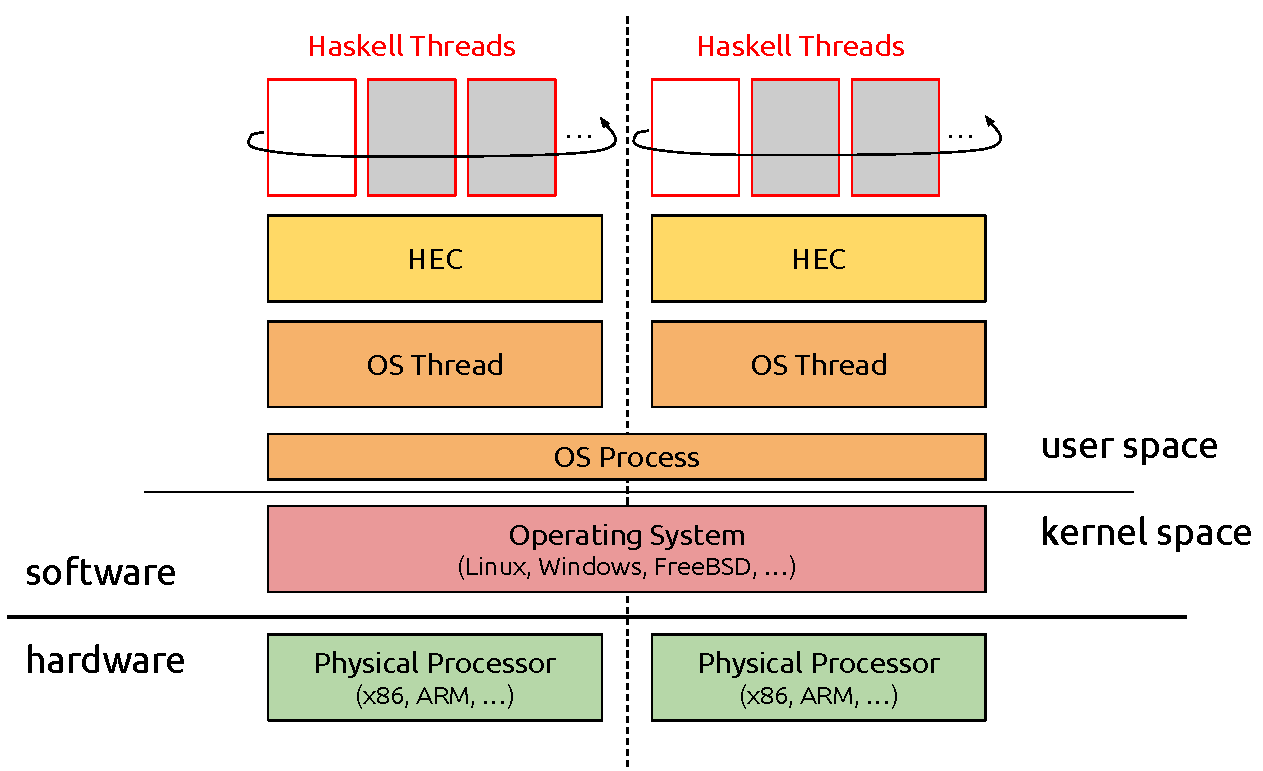
\includegraphics[width=\columnwidth]{images/haskell-concurrency-layers}
  \footnotesize{Source: Made by the author. Inspired on slides from the "GHC illustrated" presentation by Takenobu T.}
  \label{fig:haskell-conc-layers}
\end{figure}

In \figref{fig:haskell-conc-layers}, we show the various layers involved in a concurrent system written in Haskell. In this example, the underlying machine has two cores. For this reason, there are two \acp{hec} associated with two OS threads. Although depicted this way, a developer can configure it differently. For instance, the number of capabilities can be set when the program is executed  by passing a command line argument for the \ac{rts} (in this case, \texttt{-N}). Also, it is important to note that a program in Haskell can be linked with either threaded \ac{rts} or non-threaded \ac{rts}. The program should be linked to the threaded runtime to leverage multicore processors (as in \figref{fig:haskell-conc-layers}).\footnote{This can be achieved by passing \texttt{-threaded} to \ac{ghc} when compiling the program}

\begin{listing}
  \caption{The thread creation interface}
  \begin{minted}{haskell}
forkIO :: IO () -> IO ThreadId
forkOn :: Int -> IO () -> IO ThreadId
forkOS :: IO () -> IO ThreadId
  \end{minted}
  \label{code:fork-sig}
\end{listing}

From a higher-level perspective, the original framework for concurrency in Haskell is called \emph{Concurrent Haskell}~\cite{smpj:1996}. It represents a thread as a computation in the IO monad. We have three main functions to create a new thread in Haskell as \autoref{code:fork-sig} shows. \forkIO spawns a Haskell thread. It takes an IO computation to be executed concurrently and returns a pointer to the newly created thread. \forkOn also spawns a Haskell thread but lets the developer specify on which capability the thread should run. Unlike threads created with \forkIO, the scheduler cannot migrate threads created with \forkOn from one capability to another. For instance, if a program creates all its threads using \forkOn, the scheduler will not be able to perform load-balancing. Finally, \forkOS spawns a \emph{bound thread}. A bound thread is a Haskell thread that is bound to an specific OS thread. They are treated by the scheduler the same way as other Haskell threads. The only difference is when it is time to run a bound thread. The capability has to run it on its bound OS thread. \figref{fig:haskell-threads} shows the difference between each thread creation function.

\begin{figure}[htp]
  \centering
  \caption{Thread creation functions}
  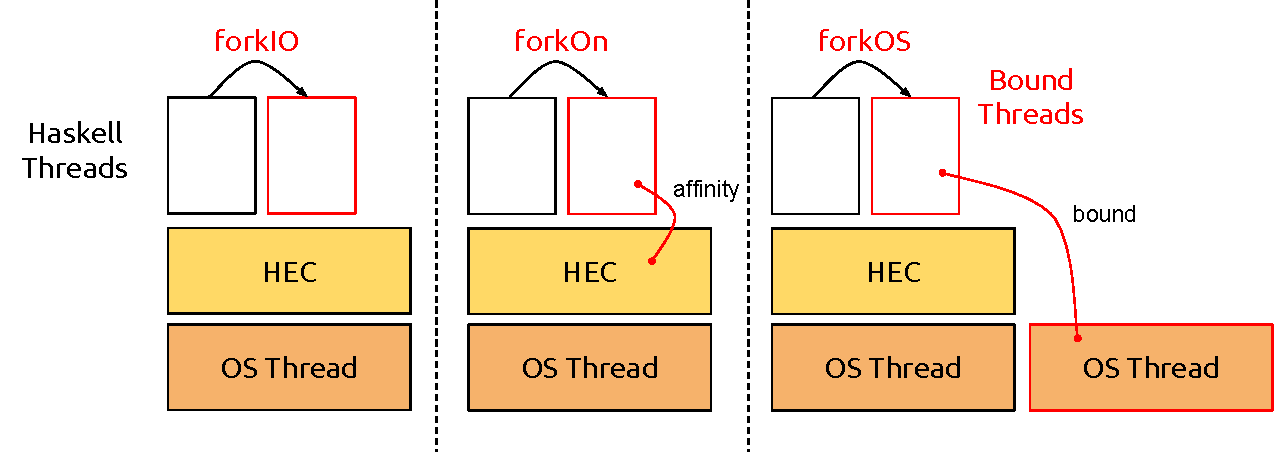
\includegraphics[width=\columnwidth]{images/haskell-threads}
  \footnotesize{Source: Made by the author. Inspired on slides from "GHC illustrated" presentation by Takenobu T.}
  \label{fig:haskell-threads}
\end{figure}

The basic concurrency control primitive of Haskell is the \MVar. A value of type \MVar~\texttt{t} is a mutable location that is either empty or contains a value of type \texttt{t}. \autoref{code:mvar-api} shows the \ac{api} for manipulating an \MVar. The more commonly used functions are \newMVar, \newEmptyMVar, \takeMVar and \putMVar. The first one creates an \MVar with a value inside. The second creates an empty \MVar. The \takeMVar function takes a value from an \MVar, returning it in the IO monad. The operation returns immediatly if the \MVar is full. For empty ones it will block until they are filled. The opposite applies to \putMVar. The function puts a value in an \MVar. It will return immediatly if the \MVar is empty. Otherwise, the function will block until the \MVar is emptied. An \MVar combines both locking and condition-based synchronization in a single primitive. It also has a formally defined semantics~\cite{smpj:1996}.

\begin{listing}
  \caption{The \MVar interface}
  \begin{minted}{haskell}
-- Type definition
data MVar a

-- MVar manipulation
takeMVar     :: MVar a -> IO a
putMVar      :: MVar a -> a -> IO ()
tryTakeMVar  :: MVar a -> IO (Maybe a)
tryPutMVar   :: MVar a -> a -> IO Bool
isEmptyMVar  :: MVar a -> IO Bool

-- MVar creation
newMVar      :: a -> IO (MVar a)
newEmptyMVar :: IO (MVar a)
  \end{minted}
  \label{code:mvar-api}
\end{listing}

In Haskell, we can also use software transactional memory to coordinate concurrency. Its implementation is called \acs{stm} Haskell~\cite{harris:2005}. \autoref{code:stm-api} shows the \acs{api} for \acs{stm} in Haskell. The transactional variable, or \TVar, is the main abstraction of this framework. A \TVar~\texttt{t} is a mutable location that holds a value of type \texttt{t}. Reads and writes to a \TVar can only be accomplished inside the \STM monad. To execute an \STM monad we have to use the \atomically function. This function runs an \STM monad as a transaction, which makes a sequence of operations to take place atomically with respect to the rest of the program. The \atomically function also acts as a bridge between the \IO and \STM monads, which allows \STM operations to be executed by threads. It is important to note that, as \STM and \IO are different monads, Haskell's type system does not allow manipulating a \TVar outside a transaction, nor does it allow performing an IO operation inside a transaction. This is an important property that is hard to ensure on other \STM implementations.

\begin{listing}
  \caption{The \STM interface}
  \begin{minted}{haskell}
-- The STM monad
data STM a
instance Monad STM -- support "do" notation and sequencing

-- Transactional variable
data TVar a
newTVar         :: a -> STM (TVar a)
readTVar        :: TVar a -> STM a
writeTVar       :: TVar a -> a -> STM ()

-- Transactional MVar
data TMVar a
newTMVar        :: a -> STM (TMVar a)
takeTMVar       :: TMVar a -> STM a
putTMVar        :: TMVar a -> a -> STM ()
tryTakeTMVar    :: TMVar a -> STM (Maybe a)
tryPutTMVar     :: TMVar a -> a -> STM Bool

-- Running STM computations
atomically      :: STM a -> IO a
retry           :: STM a
orElse          :: STM a -> STM a -> STM a
  \end{minted}
  \label{code:stm-api}
\end{listing}

In concurrent programming, it is crucial to be able to \emph{block} when we need to wait for some condition to be true. We can achieve this behavior in \acs{stm} Haskell using the \retry function. When \retry is called, the \atomically block will immediately terminate. It makes the transaction restart from scratch, with any previous modifications unperformed. The Haskell implementation is also smart enough not to restart the transaction immediately. It will do so only when one or more of the variables involved in the transaction changes. This makes it possible to block the execution of a thread on arbitrary conditions.

Having \emph{blocking} semantics also enables the creation other types, such as \TMVar. As the name implies, it works as a transactional variant of \MVar. It blocks when the \TMVar is full and we try to put a new value on it, or when the \TMVar is empty and we try to take a value from it. However, it blocks using \retry, which aborts the transaction it is in and makes it restart from the beginning. This makes the order in which the threads are woken up by the scheduler to differ between \MVar and \TMVar. \MVar functions are guaranteed to be woken up one at a time while \TMVar functions follow the retry semantics. So, while {\MVar}s are guaranteed to be fair, {\TMVar}s have no such guarantees.

As we can see, Haskell has a robust set of constructs and primitives for concurrent programming. There are several ways we can write an application to achieve a specific goal. Throughout this work, we will study how the choices we make for expressing concurrency in our Haskell programs impacts performance.


\section{Software Energy Consumption}
Energy efficiency is becoming a key software design attribute thanks to the popularity of two specific kinds of computer systems: mobile devices and data centers. We are facing a rapid proliferation of various kinds of small computers such as smartphones, tablets, and IoT sensors. In this sort of device, energy consumption is closely related to battery lifetime, so saving energy is imperative. On the data center side, we have a growth in adoption of cloud computing solutions, making many internet companies to build and manage huge data centers. In this kind of environment, due to its scale, minor energy savings can have a high impact on the maintenance costs.

Although it may seem like a recent problem, the energy efficiency of computer systems has been a concern for researchers for a long time. Initially, most of the research focused on the hardware design side, developing new ways to build electronic components that wasted less energy~\cite{chandrakasan:1992}. However, in a computer system, software plays a fundamental role in deciding how a computational task will be executed on specific hardware. For this reason, software can have a substantial impact on energy consumption.

From a software perspective, the energy efficiency problem can be tackled at different levels of abstraction, ranging from machine code level to user-facing applications. Traditionally, the research in this area has been focused on low-level software. Much progress has been achieved on building energy-efficient solutions for embedded software~\cite{tiwari:1994}, compilers~\cite{hsu:2003}, operating systems~\cite{merkel:2006} and runtime systems~\cite{ribic:2014, farkas:2000}. However, the growing worldwide movement towards sustainability, including sustainability in software~\cite{becker:2015}, have motivated the study of the energy impact of application software in execution.

Recent empirical studies have provided initial evidence that high-level decisions can effectively reduce the energy usage of an application software~\cite{chung:2001,hindle:2012,pinto:2014,trefethen:2013,manotas:2014, sahin:2012,sahin:2014}. It is important to note that optimizing software at the application level does not cancel the lower level optimizations. They are complementary solutions. However, it is still not clear which software engineering practices are beneficial for saving energy. A recent study by~\cite{pinto:2014b} shows that, although application developers are consistently more interested in understanding how to reduce energy consumption in their software, there is a general lack of information in the community about how it can be achieved.

In this work, we tackle the software energy consumption problem at the application level. Moreover, we study energy consumption in the context of Concurrent Haskell. We aim to help Haskell developers to better understand how its decisions can impact the energy consumption and performance when developing  concurrent sofware. In the next chapter, we present a first step toward this goal, which is to understand how we can measure the energy consumption of a Haskell program.
